\documentclass{beamer}
\usetheme{Madrid}
\usecolortheme{default}


\usepackage{gvv-book}
\usepackage{gvv}


\usepackage{amsmath,amssymb,amsfonts}
\usepackage{mathtools}
\usepackage{graphicx}
\usepackage{hyperref}
\usepackage{listings}
\usepackage{xcolor}


\lstset{
  basicstyle=\ttfamily\small,
  breaklines=true,
  breakatwhitespace=true,
  showstringspaces=false,
  numbers=left,
  numberstyle=\tiny,
  frame=single,
  xleftmargin=2pt,
  xrightmargin=2pt
}

% title info
\title[Q 1.6.24 --- Collinearity]{ Question 1.6.24 }
\author[AI25BTECH11009]{AI25BTECH11009 --- Dasu Harshith Kumar}
\date{\today}

\begin{document}

% title slide
\begin{frame}
  \titlepage
\end{frame}

% Problem slide
\begin{frame}{Question (1.6.24)}
\small
Find the values of \(k\) if the points
\[
A(2,3),\quad B(4,k),\quad C(6,-3)
\]
are collinear.
\end{frame}

% Solution slide 1
\begin{frame}{Solution --- set up vectors and matrix}
\small
Write position vectors:
\[
\vec{A}=\myvec{2\\3},\qquad \vec{B}=\myvec{4\\k},\qquad \vec{C}=\myvec{6\\-3}.
\]

Direction vectors:
\[
\vec{B}-\vec{A}=\myvec{2\\k-3},\qquad
\vec{C}-\vec{A}=\myvec{4\\-6}.
\]

Construct the matrix:
\[
(\vec{B}-\vec{A},\,\vec{C}-\vec{A}) = M = \myvec{2 & 4 \\ k-3 & -6}.
\]
\end{frame}

% Solution slide 2
\begin{frame}{Solution --- row reduction}
\small
\[
M \xrightarrow{R_1\leftarrow \tfrac{1}{2}R_1}
\myvec{1 & 2 \\ k-3 & -6}
\xrightarrow{R_2\leftarrow R_2 - (k-3)R_1}
\myvec{1 & 2 \\ 0 & -2k}.
\]

For collinearity, rank must be \(1\):
\[
-2k=0 \;\;\Longrightarrow\;\; k=0.
\]

\(\therefore\) The points are collinear when \(k=0\).
\end{frame}

% Conclusion + figure
\begin{frame}{Conclusion \& verification}
\small
Result: \(k=0\).

\centering
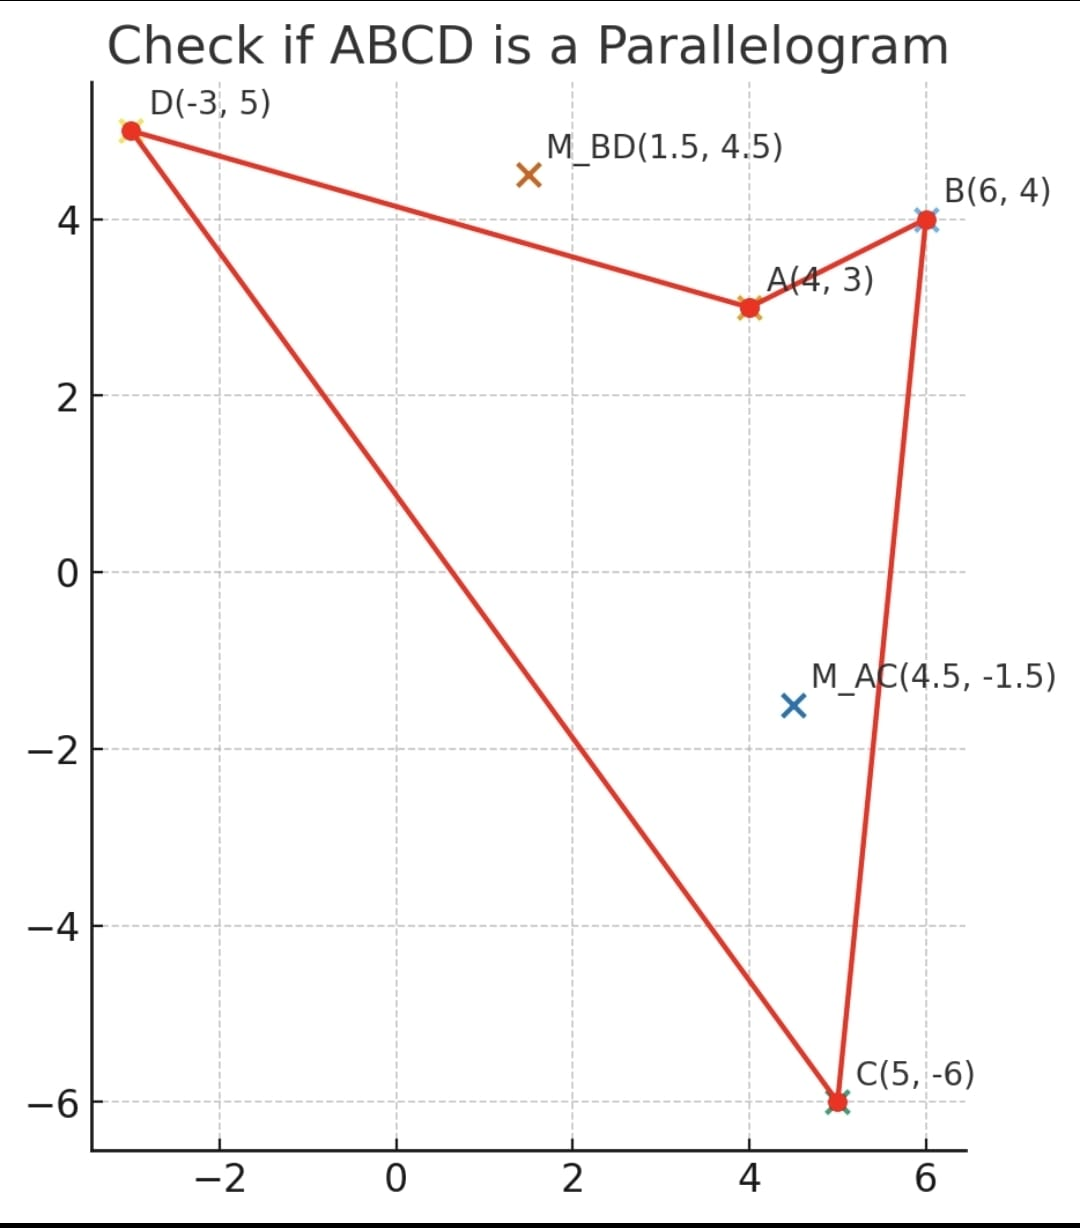
\includegraphics[width=0.65\textwidth]{figs/image1.jpg}

\footnotesize
Verification plot generated in Python.
\end{frame}

% Python code
\begin{frame}[fragile]{Python code}
\small
\begin{lstlisting}[language=Python]
import numpy as np
import matplotlib.pyplot as plt

A = np.array([2.0, 3.0])
C = np.array([6.0, -3.0])
k = 0.0
B = np.array([4.0, k])

t = np.linspace(-0.2, 1.2, 100)
line = A + np.outer(t, (C - A))

plt.figure(figsize=(6,4))
plt.plot(line[:,0], line[:,1], 'k--')
plt.plot([A[0], B[0], C[0]],
         [A[1], B[1], C[1]], 'ro')

plt.text(A[0]+0.08, A[1]+0.08, 'A')
plt.text(B[0]+0.08, B[1]+0.08, 'B')
plt.text(C[0]+0.08, C[1]+0.08, 'C')

plt.gca().set_aspect('equal', 'box')
plt.grid(True)
plt.savefig('figs/image1.jpg', dpi=300)
plt.show()
\end{lstlisting}
\end{frame}

% C code
\begin{frame}[fragile]{C code}
\small
\begin{lstlisting}[language=C]
#include <stdio.h>

int main(void) {
    double k = 0.0;
    printf("Solution: k = %.0f\n", k);
    printf("B = (4, %.0f) makes A,B,C collinear.\n", k);
    return 0;
}
\end{lstlisting}
\end{frame}

\end{document}
